\chapter{Reference Diagnostic Specifications}
\label{app:specs}

This appendix collects representative instrument specifications for the four optical diagnostic families used in the monograph -- optical emission spectroscopy (OES), laser-induced fluorescence (LIF), Thomson scattering, and interferometry -- and states the optical-access constraints a sheath-edge ion-energy-flux campaign must satisfy. The values are \emph{representative}, compiled from the literature rather than measured by the present authors, and characterise no specific instrument; they bound how precisely $T_{\mathrm{e}}$, $T_{\mathrm{i}}$, $n_{\mathrm{e}}$, $n_{\mathrm{i}}$, $\lambda_{\mathrm{D}}$, $u_{\mathrm{B}}$, and ultimately $\Gamma_{E}$ and $f_{\mathrm{i}}(v)$, can be inferred optically.

\section{Purpose and Scope of Reference Specifications}
\label{sec:specs-scope}

The main text expresses ion energy flux delivered to a plasma-facing surface as a functional of $f_{\mathrm{i}}(v)$ at the sheath edge,
\begin{equation}
\Gamma_{E} = \int_{0}^{\infty} \tfrac{1}{2} M v^{2} \, v \, f_{\mathrm{i}}(v) \, \mathrm{d}v ,
\label{eq:specs-gammaE}
\end{equation}
where $M$ is the ion mass and $f_{\mathrm{i}}(v)$ is normalised to $n_{\mathrm{i}}$. Each diagnostic supplies a partial window onto Eq.~\eqref{eq:specs-gammaE}: OES and Thomson scattering give $T_{\mathrm{e}}$ and $n_{\mathrm{e}}$, setting the Bohm speed
\begin{equation}
u_{\mathrm{B}} = \sqrt{\frac{k_{\mathrm{B}} T_{\mathrm{e}}}{M}} ,
\label{eq:specs-bohm}
\end{equation}
LIF resolves $f_{\mathrm{i}}(v)$ directly, and interferometry gives an independent, line-integrated $n_{\mathrm{e}}$ for cross-calibration. No single technique closes Eq.~\eqref{eq:specs-gammaE}; a credible determination combines at least two diagnostics sharing a calibration and a measurement volume referenced to the Debye length
\begin{equation}
\lambda_{\mathrm{D}} = \sqrt{\frac{\varepsilon_{0} k_{\mathrm{B}} T_{\mathrm{e}}}{n_{\mathrm{e}} e^{2}}} .
\label{eq:specs-debye}
\end{equation}

\section{Optical Emission Spectroscopy}
\label{sec:specs-oes}

OES is the least invasive, least expensive of the four, needing only a single collection optic and no probe beam. It returns line-integrated rather than localised information unless combined with Abel inversion, and its $T_{\mathrm{e}}$/$n_{\mathrm{e}}$ inference depends on a CR model rather than a first-principles relation \cite{ref0231,ref0237}.

\subsection{Spectrometer and Detector Architecture}

Representative OES systems use a Czerny--Turner spectrograph coupled to the plasma via a fibre bundle with $\mathrm{NA} \approx 0.1$--$0.22$. Angular dispersion follows the grating equation,
\begin{equation}
m \lambda = d \left( \sin\theta_{i} + \sin\theta_{d} \right) ,
\label{eq:specs-grating}
\end{equation}
with $m$ the diffraction order, $d$ the groove spacing, $\theta_{i}$, $\theta_{d}$ the incidence/diffraction angles. Differentiating at fixed $\theta_{i}$ and combining with focal length $f$ gives the reciprocal linear dispersion,
\begin{equation}
\mathcal{R} \equiv \frac{\mathrm{d}\lambda}{\mathrm{d}x} \approx \frac{d \cos\theta_{d}}{m f} ,
\label{eq:specs-dispersion}
\end{equation}
typically $\sim\SI{1}{\nano\meter\per\milli\meter}$ for a $\SI{0.5}{\meter}$ instrument with an $\SI{1800}{grooves\per\milli\meter}$ grating, though slit width and pixel sampling set the practical instrument function.

Detection uses a back-illuminated CCD/sCMOS for survey work, a gated ICCD/PMT for fast transients such as sheath formation \cite{ref0256}, or a photon-counting PMT for photometric accuracy.

\subsection{Line Selection and Collisional-Radiative Inference}

Since OES does not measure a velocity distribution, $T_{\mathrm{e}}$ and $n_{\mathrm{e}}$ are inferred from line intensities via a CR model balancing electron-impact excitation, radiative decay, and de-excitation \cite{ref0237,ref0245}. For a thin, steady-state level $p$, transition $p \to q$ intensity scales as
\begin{equation}
I_{pq} \; \propto \; n_{\mathrm{e}} \, n_{0} \, \langle \sigma_{pq}^{\mathrm{exc}} v_{\mathrm{e}} \rangle \, A_{pq} \Big/ \sum_{r<p} A_{pr} ,
\label{eq:specs-crmodel}
\end{equation}
where $n_{0}$ is the ground-state density, $\langle \sigma_{pq}^{\mathrm{exc}} v_{\mathrm{e}} \rangle$ the Maxwellian-averaged excitation rate coefficient, and $A_{pq}$ the spontaneous emission coefficient. The ratio of two lines with different upper-level energies cancels $n_{\mathrm{e}} n_{0}$, giving a ratio monotonic in $T_{\mathrm{e}}$ alone and invertible against a CR grid; a second line pair then returns $n_{\mathrm{e}}$ \cite{ref0231}.

\subsection{Representative OES Specification Table}

\begin{table}[htbp]
\centering
\caption{Representative (illustrative, non-measured) optical emission spectroscopy specifications.}
\label{tab:oes-specs}
\begin{tabular}{@{}ll@{}}
\toprule
Parameter & Representative value \\
\midrule
Spectrometer architecture & Czerny--Turner / crossed Czerny--Turner \\
Focal length & \SI{0.3}{\meter} -- \SI{1.0}{\meter} \\
Grating groove density & \SIrange{300}{2400}{grooves\per\milli\meter} \\
Spectral coverage & \SIrange{200}{1000}{\nano\meter} \\
Spectral resolution (FWHM) & \SIrange{0.02}{0.15}{\nano\meter} \\
Entrance-slit width & \SIrange{10}{100}{\micro\meter} \\
Collection optic & Fibre bundle, $\mathrm{NA} \approx 0.10$--$0.22$ \\
Detector & Back-illuminated CCD / sCMOS / ICCD / PMT \\
Quantum efficiency (peak) & \SIrange{40}{95}{\percent} \\
Dynamic range & $10^{3}$--$10^{5}$ (16-bit typical) \\
Minimum gate width (ICCD) & \SIrange{2}{5}{\nano\second} \\
Typical integration time & \SIrange{1}{1000}{\milli\second} \\
Spatial resolution along l.o.s. & \SIrange{1}{5}{\milli\meter} (fibre-limited) \\
\bottomrule
\end{tabular}
\end{table}

\section{Laser-Induced Fluorescence}
\label{sec:specs-lif}

LIF most directly targets $f_{\mathrm{i}}(v)$: a narrow-linewidth, frequency-scanned laser is tuned across an ionic (or, for two-photon LIF, atomic) transition, and fluorescence intensity vs.\ frequency reproduces the Doppler-broadened absorption profile, proportional to the projection of $f_{\mathrm{i}}(v)$ along the laser $k$-vector \cite{ref0292,ref0300}. Spatially localised and needing no equilibrium assumption, it suits non-Maxwellian, sheath-accelerated ions \cite{ref0304,ref0322}.

\subsection{Laser Source and Tuning}

Representative LIF systems for singly ionised noble gases (e.g.\ ArII near $\SI{670}{\nano\meter}$) use external-cavity/distributed-feedback diode lasers, or CW ring dye/Ti:sapphire lasers outside the diode band, with mode-hop-free tuning over $\SIrange{10}{60}{\giga\hertz}$ and linewidth below the Doppler width. The Doppler FWHM for an ion of mass $M$ at temperature $T_{\mathrm{i}}$ is
\begin{equation}
\Delta\nu_{\mathrm{D}} = \frac{\nu_{0}}{c} \sqrt{\frac{8 \ln 2 \, k_{\mathrm{B}} T_{\mathrm{i}}}{M}} ,
\label{eq:specs-doppler}
\end{equation}
giving $\Delta\nu_{\mathrm{D}} \sim \SI{3}{\giga\hertz}$ for Ar$^{+}$ at $T_{\mathrm{i}} \sim \SI{0.3}{\electronvolt}$, resolved by a $\lesssim \SI{10}{\mega\hertz}$ laser. Irradiance must stay below saturation ($\sim\SI{1}{\milli\watt\per\milli\meter\squared}$) to avoid power broadening.

\subsection{Excitation Scheme and Detection}

The pump beam is chopped at a few kHz to tens of kHz, and fluorescence is demodulated with a lock-in amplifier or gated photon counter, suppressing unmodulated self-emission \cite{ref0300,ref0304}. The fluorescence photon, on a decay branch distinct from the pump wavelength, is detected by a PMT or avalanche photodiode behind an interference filter. TALIF, needed for ground-state species, uses pulsed, frequency-multiplied sources with extra Rabi/photoionisation-loss constraints. Spatial resolution is set by the pump-beam waist (typically $\SIrange{0.2}{1}{\milli\meter}$) and the collection field of view, usually at $\SI{90}{\degree}$ to minimise scattered light.

\subsection{Representative LIF Specification Table}

\begin{table}[htbp]
\centering
\caption{Representative (illustrative, non-measured) laser-induced fluorescence specifications.}
\label{tab:lif-specs}
\begin{tabular}{@{}ll@{}}
\toprule
Parameter & Representative value \\
\midrule
Laser type & External-cavity / distributed-feedback diode, or CW ring dye \\
Tuning range (mode-hop-free) & \SIrange{10}{60}{\giga\hertz} \\
Intrinsic laser linewidth & \SIrange{1}{10}{\mega\hertz} \\
Typical pump wavelength & \SIrange{375}{800}{\nano\meter} (species-dependent) \\
Output power (CW single-photon LIF) & \SIrange{10}{200}{\milli\watt} \\
Pulse energy (TALIF, pulsed) & \SIrange{0.1}{5}{\milli\joule} per pulse \\
Beam waist at focus & \SIrange{0.2}{1.0}{\milli\meter} \\
Modulation / chop frequency & \SIrange{1}{50}{\kilo\hertz} \\
Detector & PMT or avalanche photodiode \\
Spectral discrimination & Interference filter, $\Delta\lambda \sim \SIrange{1}{10}{\nano\meter}$ \\
Signal recovery & Lock-in amplifier / gated photon counting \\
Achievable velocity resolution & $\lesssim \SI{100}{\meter\per\second}$ \\
Spatial resolution & \SIrange{0.2}{2}{\milli\meter} \\
\bottomrule
\end{tabular}
\end{table}

\section{Thomson Scattering}
\label{sec:specs-thomson}

Thomson scattering alone provides $T_{\mathrm{e}}$ and $n_{\mathrm{e}}$ from a first-principles cross section, independent of any atomic model or branching ratios \cite{ref0354,ref0384}. Its cost is the tiny differential cross section of free-electron scattering,
\begin{equation}
\frac{\mathrm{d}\sigma_{\mathrm{T}}}{\mathrm{d}\Omega} = r_{\mathrm{e}}^{2} \sin^{2}\chi , \qquad \sigma_{\mathrm{T}} = \frac{8\pi}{3} r_{\mathrm{e}}^{2} \approx \SI{6.652e-29}{\meter\squared} ,
\label{eq:specs-thomson-xsec}
\end{equation}
where $r_{\mathrm{e}} = e^{2}/(4\pi\varepsilon_{0} m_{\mathrm{e}} c^{2}) \approx \SI{2.818e-15}{\meter}$ is the classical electron radius and $\chi$ the polarisation-observation angle. Eight orders of magnitude smaller than Rayleigh cross sections, it demands a high-energy probe laser, low-stray-light optics, and absolute Raman/Rayleigh calibration in a reference gas \cite{ref0357,ref0362}.

\subsection{Scattering Geometry and Cross Section}

The scattering wavevector $\vec{k} = \vec{k}_{\mathrm{s}} - \vec{k}_{\mathrm{i}}$ has magnitude $k = (4\pi/\lambda_{0}) \sin(\theta/2)$, and the dimensionless parameter
\begin{equation}
\alpha \equiv \frac{1}{k \lambda_{\mathrm{D}}}
\label{eq:specs-alpha}
\end{equation}
sets the regime: for $\alpha \ll 1$ (non-collective) the spectrum reproduces the electron velocity distribution along $\vec{k}$, with Doppler width
\begin{equation}
\Delta\lambda_{1/e} \approx \frac{2\lambda_{0}}{c} \sin\!\left(\frac{\theta}{2}\right) \sqrt{\frac{2 k_{\mathrm{B}} T_{\mathrm{e}}}{m_{\mathrm{e}}}} ,
\label{eq:specs-thomson-doppler}
\end{equation}
from which $T_{\mathrm{e}}$ follows by spectral fit and $n_{\mathrm{e}}$ from the absolute scattered power once calibrated. For $\alpha \gtrsim 1$ (collective), satellites encode $n_{\mathrm{e}}$, $T_{\mathrm{e}}$, $T_{\mathrm{i}}$ jointly; values below assume non-collective scattering.

\subsection{Laser and Collection Optics}

Representative systems use a pulsed, frequency-doubled Nd:YAG laser at $\SI{532}{\nano\meter}$ (or $\SI{1064}{\nano\meter}$) delivering $\SIrange{100}{1000}{\milli\joule}$ in $\SIrange{5}{10}{\nano\second}$ pulses, focused to a few-hundred-micrometre waist \cite{ref0357}. Collection optics sit at $\SI{90}{\degree}$ to the laser to minimise stray light, imaged onto a triple-grating or subtractive-dispersion spectrometer for rejection at the laser wavelength, since the Doppler-shifted signal lies within a few nanometres of it in cold plasmas. Detection is a gated ICCD synchronised to the pulse with nanosecond jitter, rejecting self-emission \cite{ref0362}.

\subsection{Representative Thomson Scattering Specification Table}

\begin{table}[htbp]
\centering
\caption{Representative (illustrative, non-measured) Thomson scattering diagnostic specifications.}
\label{tab:thomson-specs}
\begin{tabular}{@{}ll@{}}
\toprule
Parameter & Representative value \\
\midrule
Laser & Pulsed Nd:YAG, \SI{532}{\nano\meter} (2$\omega$) or \SI{1064}{\nano\meter} \\
Pulse energy & \SIrange{100}{1000}{\milli\joule} \\
Pulse duration & \SIrange{5}{10}{\nano\second} \\
Repetition rate & \SIrange{10}{30}{\hertz} (up to \SI{20}{\kilo\hertz} for burst systems) \\
Focal spot diameter & \SIrange{100}{500}{\micro\meter} \\
Scattering angle & \SI{90}{\degree} (typical) \\
Collection $f$-number & $f/4$ -- $f/10$ \\
Spectrometer & Triple-grating / subtractive-dispersion, stray-light rejection $\gtrsim 10^{-13}$ \\
Detector & Gated ICCD, gate width \SIrange{5}{20}{\nano\second} \\
Absolute calibration method & Rotational Raman or Rayleigh scattering in reference gas \\
Accessible $T_{\mathrm{e}}$ range & \SIrange{0.1}{100}{\electronvolt} \\
Accessible $n_{\mathrm{e}}$ range & $10^{17}$ -- $10^{21}\ \si{\per\meter\cubed}$ \\
Spatial resolution & \SIrange{0.1}{1}{\milli\meter} (laser-waist limited) \\
\bottomrule
\end{tabular}
\end{table}

\section{Interferometry}
\label{sec:specs-interferometry}

Interferometry measures the plasma's contribution to refractive index along a probe chord, unique among the four in needing no photometric calibration or atomic model: the observable is a phase shift, with uncertainty set by mechanical/vibrational stability rather than cross sections \cite{ref0391}. Its limitation is that this observable is a line integral of $n_{\mathrm{e}}$, requiring multi-chord tomography or an assumed symmetry for spatial resolution.

\subsection{Phase-Shift Principle}

For a probe wave of angular frequency $\omega$ through an unmagnetised plasma of density $n_{\mathrm{e}}(\vec{r})$, the refractive index is
\begin{equation}
\eta(\vec{r}) = \sqrt{1 - \frac{\omega_{\mathrm{pe}}^{2}(\vec{r})}{\omega^{2}}} \approx 1 - \frac{n_{\mathrm{e}}(\vec{r})}{2 n_{\mathrm{c}}} , \qquad n_{\mathrm{c}} = \frac{\varepsilon_{0} m_{\mathrm{e}} \omega^{2}}{e^{2}} ,
\label{eq:specs-refractive-index}
\end{equation}
valid for $n_{\mathrm{e}} \ll n_{\mathrm{c}}$, the critical density. Comparing the phase along a chord of length $L$ against a vacuum reference gives
\begin{equation}
\Delta\varphi = \frac{2\pi}{\lambda} \int_{0}^{L} \bigl[1 - \eta(\vec{r})\bigr] \, \mathrm{d}\ell \; \approx \; \frac{e^{2}\lambda}{4\pi \varepsilon_{0} m_{\mathrm{e}} c^{2}} \int_{0}^{L} n_{\mathrm{e}} \, \mathrm{d}\ell \; = \; r_{\mathrm{e}} \lambda \int_{0}^{L} n_{\mathrm{e}} \, \mathrm{d}\ell ,
\label{eq:specs-phase-shift}
\end{equation}
i.e.\ the phase shift is proportional to the line-integrated density and to $\lambda$. Long-wavelength (far-infrared/THz/microwave) interferometers thus suit low-density plasmas, while visible-wavelength interferometry suits denser laser-produced or pulsed-power plasmas \cite{ref0400}.

\subsection{Configurations}

Representative configurations include two-beam Mach--Zehnder/Michelson layouts, recombining a probe beam with an unperturbed reference, and heterodyne (dispersion) interferometers, converting a small frequency offset into a beat-frequency measurement insensitive to vibration \cite{ref0400}. Multi-chord systems permit tomographic (Abel) inversion to a radially resolved $n_{\mathrm{e}}(r)$; single-chord systems return only path-integrated density, commonly cross-validated against Thomson scattering \cite{ref0391}.

\subsection{Representative Interferometry Specification Table}

\begin{table}[htbp]
\centering
\caption{Representative (illustrative, non-measured) interferometry diagnostic specifications.}
\label{tab:interferometry-specs}
\begin{tabular}{@{}ll@{}}
\toprule
Parameter & Representative value \\
\midrule
Configuration & Mach--Zehnder / Michelson / heterodyne (dispersion) \\
Probe wavelength & \SI{632.8}{\nano\meter} (HeNe) to \SI{10.6}{\micro\meter} (CO$_2$), or mm-wave/THz \\
Number of chords & 1 (single-chord) to $\sim$16 (tomographic) \\
Phase resolution & $2\pi/100$ -- $2\pi/1000$ rad \\
Minimum detectable line-integrated $n_{\mathrm{e}}$ & $10^{16}$ -- $10^{18}\ \si{\per\meter\squared}$ \\
Time resolution & \SIrange{0.1}{10}{\micro\second} \\
Detector & Photodiode / pyroelectric / Schottky mixer (frequency-dependent) \\
Path-length stability requirement & $\ll \lambda/10$ over acquisition window \\
Spatial resolution (tomographic) & \SIrange{1}{10}{\milli\meter} (inversion-limited) \\
\bottomrule
\end{tabular}
\end{table}

\section{Optical Access and Integration Requirements}
\label{sec:specs-integration}

Deploying two or more diagnostics on one test article to close Eq.~\eqref{eq:specs-gammaE} imposes mechanical, optical, and timing constraints beyond any single instrument.

\subsection{Viewport and Standoff Constraints}

Every diagnostic volume must sit far enough from the plasma-facing surface to sample the quasi-neutral bulk or presheath, rather than the space-charge sheath whose thickness $s$ collapses toward the wall on the scale of $\lambda_{\mathrm{D}}$. For a planar, collisionless sheath, Child-law scaling gives normalised thickness vs.\ potential drop $\eta \equiv eV_{0}/(k_{\mathrm{B}} T_{\mathrm{e}})$,
\begin{equation}
\frac{s}{\lambda_{\mathrm{D}}} \; \approx \; \frac{\sqrt{2}}{3} \, (2\eta)^{3/4} ,
\label{eq:specs-childlaw}
\end{equation}
which grows only as $\eta^{3/4}$ but reaches several tens of Debye lengths for $\eta \sim 10^{2}$--$10^{3}$, typical of RF-biased surfaces (Fig.~\ref{fig:childlaw-sheath}), motivating the standoff distances in Table~\ref{tab:integration-specs}.

\begin{figure}[htbp]
\centering
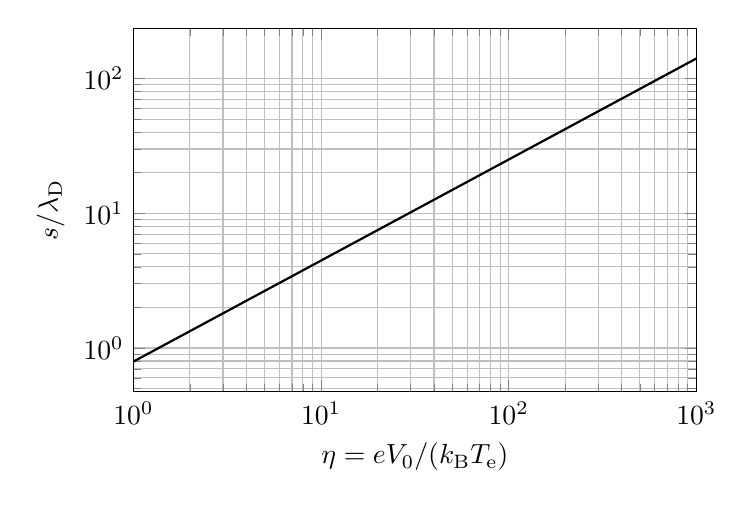
\begin{tikzpicture}
\begin{axis}[
 width=0.72\textwidth,
 height=6.2cm,
 xmode=log, ymode=log,
 xlabel={$\eta = eV_{0}/(k_{\mathrm{B}} T_{\mathrm{e}})$},
 ylabel={$s/\lambda_{\mathrm{D}}$},
 grid=both,
 domain=1:1000,
 samples=120,
 xmin=1, xmax=1000,
 axis lines=box,
]
\addplot[thick, black] {(sqrt(2)/3)*(2*x)^(0.75)};
\end{axis}
\end{tikzpicture}
\caption{Analytic Child-law scaling of the collisionless planar sheath thickness $s/\lambda_{\mathrm{D}}$ (Eq.~\eqref{eq:specs-childlaw}); motivates the standoff distances in Table~\ref{tab:integration-specs}. Not measured data.}
\label{fig:childlaw-sheath}
\end{figure}

Measurement volumes should sit at least several sheath thicknesses -- typically $\SIrange{1}{10}{\milli\meter}$ here -- from the wall, so the sampled population is unperturbed presheath or bulk plasma. Figure~\ref{fig:optical-access-schematic} sketches how the four beams can be arranged around a common volume at this standoff.

\begin{figure}[htbp]
\centering
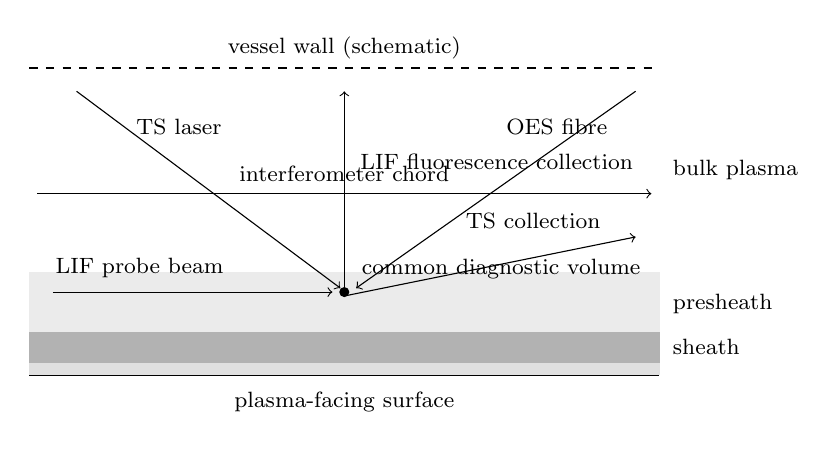
\begin{tikzpicture}[scale=1.0, every node/.style={font=\footnotesize}]
 \draw[very thick] (-4,0) -- (4,0);
 \filldraw[black!12] (-4,0) rectangle (4,0.15);
 \node at (0,-0.35) {plasma-facing surface};
 \filldraw[black!30] (-4,0.15) rectangle (4,0.55);
 \node[anchor=west] at (4.05,0.35) {sheath};
 \filldraw[black!8] (-4,0.55) rectangle (4,1.3);
 \node[anchor=west] at (4.05,0.9) {presheath};
 \node[anchor=west] at (4.05,2.6) {bulk plasma};
 \filldraw[black] (0,1.05) circle (1.6pt);
 \node[anchor=south west] at (0.1,1.1) {common diagnostic volume};
 \draw[->] (3.7,3.6) -- (0.15,1.1);
 \node at (2.7,3.15) {OES fibre};
 \draw[->] (-3.7,1.05) -- (-0.15,1.05);
 \node at (-2.6,1.35) {LIF probe beam};
 \draw[->] (0,1.05) -- (0,3.6);
 \node[anchor=west] at (0.08,2.7) {LIF fluorescence collection};
 \draw[->] (-3.4,3.6) -- (-0.05,1.1);
 \node at (-2.1,3.15) {TS laser};
 \draw[->] (0,1.0) -- (3.7,1.75);
 \node at (2.4,1.95) {TS collection};
 \draw[->] (-3.9,2.3) -- (3.9,2.3);
 \node at (0,2.55) {interferometer chord};
 \draw[thick, dashed] (-4,3.9) -- (4,3.9);
 \node at (0,4.15) {vessel wall (schematic)};
\end{tikzpicture}
\caption{Schematic (not to scale) optical access for the four diagnostics about a common measurement volume beyond the sheath, in the presheath/bulk plasma. Indicative only.}
\label{fig:optical-access-schematic}
\end{figure}

Windows must transmit every wavelength in simultaneous use (materials in Table~\ref{tab:integration-specs}); in sputtering environments a shutter, gas curtain, or sacrificial flat should protect them from film buildup.

\subsection{Synchronization and Multi-Diagnostic Integration}

Operating pulsed diagnostics (Thomson scattering, pulsed LIF/TALIF) alongside continuous ones (OES, CW LIF, interferometry) requires a common timing reference with jitter well below the shortest timescale of interest -- typically the RF period or ion-transit time across the sheath. A representative budget (Table~\ref{tab:integration-specs}) ranges from $\lesssim \SI{1}{\nano\second}$, synchronising the Thomson laser Q-switch to the ICCD gate, to $\lesssim \SI{1}{\micro\second}$ for aligning OES/interferometer acquisition. Cross-calibration matters equally: absolute density from Thomson scattering and line-integrated density from interferometry (Eq.~\eqref{eq:specs-phase-shift}) give two independent routes to $n_{\mathrm{e}}$, checked for agreement before combining OES-inferred $T_{\mathrm{e}}$ with LIF-inferred $f_{\mathrm{i}}(v)$ in Eq.~\eqref{eq:specs-gammaE}.

\subsection{Representative Integration Requirements Table}

\begin{table}[htbp]
\centering
\caption{Representative (illustrative, non-measured) optical-access and integration requirements.}
\label{tab:integration-specs}
\begin{tabular}{@{}ll@{}}
\toprule
Requirement & Representative value \\
\midrule
Minimum diagnostic-volume standoff from wall & \SIrange{1}{10}{\milli\meter} ($\gtrsim$ several $\lambda_{\mathrm{D}}$--$s$) \\
Window material (visible/UV instruments) & Fused silica / UV-grade sapphire \\
Window material (IR/THz interferometry) & ZnSe / crystal quartz / polyethylene \\
Anti-reflection coating requirement & $R < \SI{0.5}{\percent}$ per surface at operating $\lambda$ \\
Viewport count (minimum, 4-diagnostic system) & 6--8 (probe + collection per instrument) \\
Cross-trigger timing jitter (pulsed instruments) & $\lesssim \SI{1}{\nano\second}$--\SI{10}{\nano\second} \\
Cross-trigger timing jitter (CW/slow instruments) & $\lesssim \SI{1}{\micro\second}$ \\
Mechanical vibration tolerance (interferometry) & $\ll \lambda_{\mathrm{probe}}/10$ path-length change \\
Density cross-check tolerance (Thomson vs.\ interferometry) & Agreement within combined $1\sigma$ uncertainty \\
Window contamination mitigation & Shutter / gas curtain / sacrificial flat \\
\bottomrule
\end{tabular}
\end{table}

\section{Summary}
\label{sec:specs-summary}

This appendix has assembled representative specifications for the four diagnostics providing the observational basis for the sheath-edge quantities entering $\Gamma_{E}$. OES offers the least invasive, least costly route to $T_{\mathrm{e}}$ and $n_{\mathrm{e}}$ but depends on a CR model; LIF alone resolves $f_{\mathrm{i}}(v)$ directly, at the cost of a narrow-linewidth, transition-matched laser; Thomson scattering returns $T_{\mathrm{e}}$ and $n_{\mathrm{e}}$ independent of atomic structure, at the cost of a weak signal needing a high-energy laser and stray-light-optimised collection; and interferometry supplies an independently calibrated, line-integrated density as cross-check. None of the values in Tables~\ref{tab:oes-specs}--\ref{tab:integration-specs}, nor the curves in Figs.~\ref{fig:childlaw-sheath} and \ref{fig:optical-access-schematic}, are measured data; they size the infrastructure for a coherent campaign.
